\documentclass[]{article}
\usepackage{fullpage, amsmath}


\usepackage{graphicx}
\graphicspath{{../../data/05_reporting/problem_set_2/}}

%opening
\title{STAT 6300 Problem Set \#2}
\author{Anthony Barrows, Nicholas Thielsen, Lute Lillo}

\begin{document}

\maketitle


\section{Short Answers}

\subsection{Voting Records}
\begin{figure}[H]
    \centering
    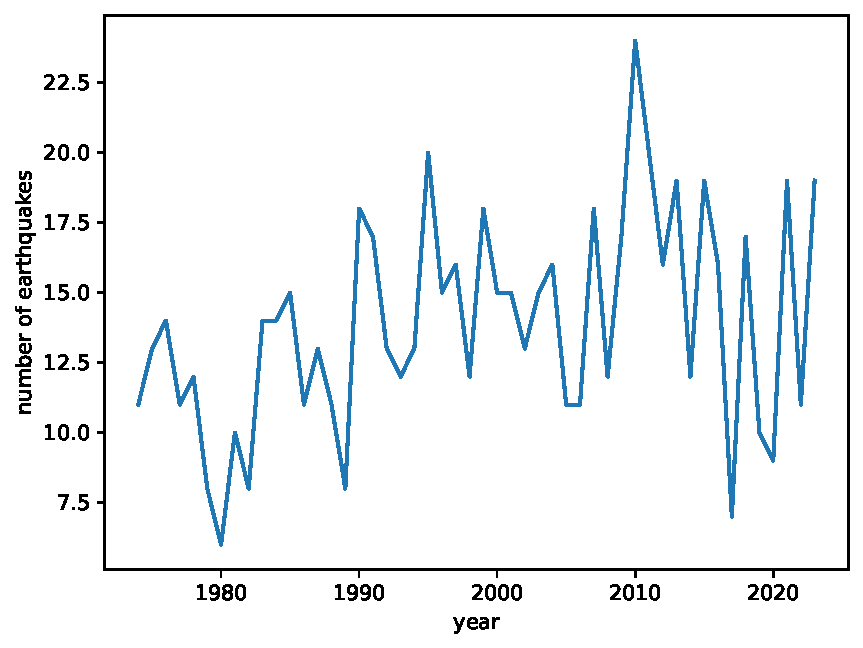
\includegraphics[width=0.5\linewidth]{data/05_reporting/problem_set_3/quake_counts.pdf}
    \caption{USGS Earthquake Hazard Program counts of earthquakes with magnitude 7.0 or higher between January 1, 1974 and December 31, 2023.}
    \label{fig:quake-counts}
\end{figure}

\subsection{Computational Complexity Code}
The number of evaluations of the posterior distribution is determined from the number of parameters which that the posterior distribution depends on, and their sampling. In this case, the posterior distribution depends on parameters $\alpha$, $\beta$, and $\sigma$, and each parameter uses a sampling resolution of 10, so the number of evaluations of the posterior distribution is $n^3=10^3=1000$. We are making the assumption here that the parameters are independent, i.e. their sampling is independent.

\subsection{Convergence Diagnostics}
\subsection{}
\begin{minted}{python}
def grid_approx_posterior(Y: pd.Series, alpha=14, beta=4):
   # define a grid of possible values for lambda
   # construct distribution for lambda using gamma prior
   a = alpha
   scale = 1 / beta

   prior = sps.gamma(a, scale=scale).logpdf(grid_lambda)
   
   likelihoods = [sps.poisson(mu = grid_lambda).logpmf(y) for y in Y]
   likelihood = np.sum(np.vstack(likelihoods), axis=0)
   
   posterior = np.exp(likelihood + prior)
   normalized = posterior / sum(posterior)

   return normalized / sum(normalized)

grid_lambda = np.linspace(10, 15, num=100)
grid_posterior = grid_approx_posterior(Y, alpha, beta)

# need to normalize twice because of floating point precision
grid_samples = np.random.choice(grid_lambda, 
                                 size=5000, 
                                 p=grid_posterior/np.sum(grid_posterior))
    
\end{minted}

\section{Bayesian Decision Theory}

\subsection{Setting up the Problem}
The likelihood is defined as the probability of data $X$ given a parameter (e.g., $\theta$). $X_i$ is a random variable distributed according to a normal distribution, meaning the first line

\[
    X_i \sim \text{Normal}(\mu, \sigma^2)
\]

describes the likelihood.

\subsection{Optimization Equation}
Considering first the left term of the RHS of the equation in 2.1:
\begin{align*}
    & \frac{d}{du}\int_{-\infty}^{u} k_1(u-\theta)\cdot p(\theta=t|X)d\theta\\
   &= k_1(u-u)\cdot p(u=t|X)\cdot \frac{d}{du}u - \lim_{q\rightarrow-\infty} k_1(u-q)\cdot p(q=t|X)\cdot \frac{d}{du}q + \int_{-\infty}^{u} \frac{\partial}{\partial u} k_1(u-\theta)\cdot p(\theta=t|X)d\theta\\
   &= 0 - 0 + \int_{-\infty}^{u} k_1\cdot p(\theta=t|X) d\theta \text{ (since $u-u=0$ in the first term and $\frac{d}{du}q=0$ in the second term)}\\
   &= k_1 \int_{-\infty}^{u} p(\theta=t|X) d\theta
\end{align*}
Now considering the right term of the RHS of the equation in 2.1:
\begin{align*}
    & \frac{d}{du}\int_{u}^{\infty} k_2(\theta-u)\cdot p(\theta=t|X)d\theta\\
   &= \lim_{q\rightarrow\infty} k_2(q-u)\cdot p(q=t|X)\cdot \frac{d}{du}q - k_2(u-u)\cdot p(u=t|X)\cdot \frac{d}{du}u + \int_{u}^{\infty} \frac{\partial}{\partial u} k_2(\theta-u)\cdot p(\theta=t|X)d\theta\\
   &= 0 - 0 - \int_{u}^{\infty} k_2\cdot p(\theta=t|X) d\theta \text{ (since $\frac{d}{du}q=0$ in the first term and $u-u=0$ in the second term)}\\
   &= -k_2 \int_{u}^{\infty} p(\theta=t|X) d\theta\\
   &= -k_2 \left(1-\int_{-\infty}^{u} p(\theta=t|X)d\theta\right)\\
   &= k_2 \left(\int_{-\infty}^{u} p(\theta=t|X)d\theta-1\right)
\end{align*}
Thus, the full expression becomes:
\begin{align*}
    0 &= k_1 \int_{-\infty}^{u} p(\theta=t|X) d\theta + k_2 \left(\int_{-\infty}^{u} p(\theta=t|X)d\theta-1\right)\\
    0 &= (k_1 + k_2)\int_{-\infty}^{u} p(\theta=t|X) d\theta - k_2
\end{align*}

\subsection{Algebraic Manipulations}
Using the distribution function of $p(\theta|X)$ (i.e., the CDF), $\int_{-\infty}^{u} p(\theta=t|X) d\theta$ becomes $F_\theta(\hat{u})$, and we have the following:
\begin{align*}
    0 &= (k_1 + k_2)\cdot F_\theta(\hat{u}) - k_2\\
    k_2 &= (k_1 + k_2)\cdot F_\theta(\hat{u})\\
    F_\theta(\hat{u}) &= \frac{k_2}{k_1+k_2}
\end{align*}

\subsection{Is the Optimum a Minimum?}
Taking another derivative with respect to u, we have:
\begin{align*}
    & \frac{d}{du}(k_1+k_2)\cdot F_\theta(\hat{u}) - k_2 = (k_1+k_2)\cdot f_\theta(\hat{u}) > 0\\
    & \text{ (since every pdf $>0$ and $k_1$ and $k_2$ are non-negative)}
\end{align*}
When the second derivative of some function equals zero, there is an inflection point since the slope changes from increasing to decreasing or vice versa. When the second derivative is less than zero, the slope is decreasing, which corresponds to concave down regions. Finally, when the second derivative is greater than zero, the slope is increasing, which corresponds to concave up regions. Whereas a maximum can only occur in a concave down region, a minimum can only occur in a concave up region. Thus, a positive second derivative is a requirement for a minimum at a particular location and it also rules out a maximum at that location.

\subsection{Usage}
Using the result of the first derivative equal to zero, we can plug in any pair $k_1, k_2$ and use the inverse CDF of the histogram for the given data to determine the estimator that minimizes the expected loss. That is to say the following:
\begin{align*}
    \hat{u} = F_\theta^{-1}\left(\frac{k_2}{k_1+k_2}\right)
\end{align*}

Thus, with $(k_1, k_2) = (20, 40)$, we determine an estimator $\mathbf{\hat{u}=20.56}$ for 50 bins in the CDF:
\begin{center}
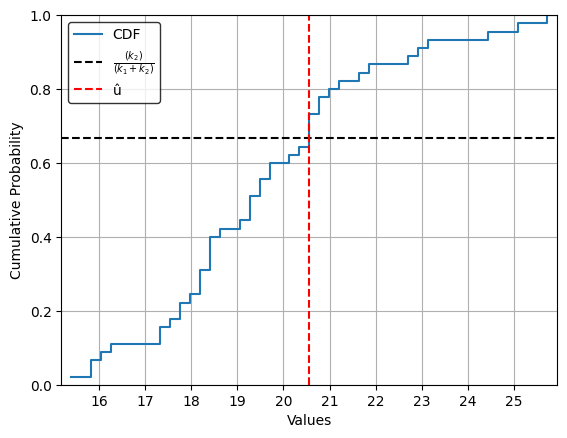
\includegraphics[scale=0.8]{data/05_reporting/problem_set_2/pset2p2.5.1.png}
\end{center}

Next, with $(k_1, k_2) = (0.5, 6)$, we determine an estimator $\mathbf{\hat{u}=23.14}$ for 50 bins in the CDF:
\begin{center}
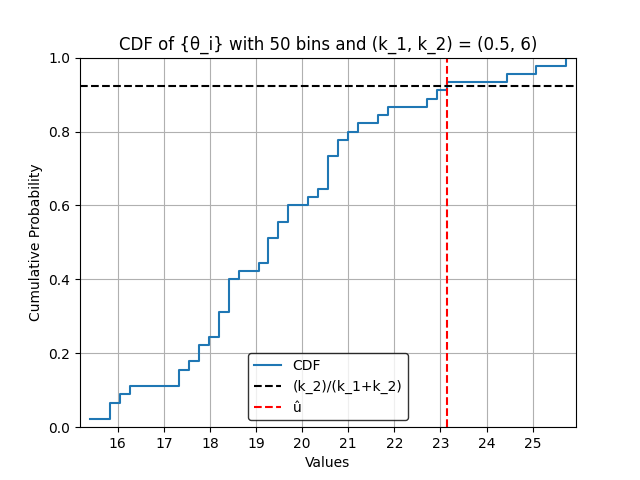
\includegraphics[scale=0.8]{data/05_reporting/problem_set_2/pset2p2.5.2.png}
\end{center}


\subsection{A Curious Result (Optional)}

\section{Data Analysis: Linear Penguins}

\subsection{Data Preparation}

\subsection{Model Formulation}
Our selected priors are:\\
\begin{align*}
    \alpha &\sim \text{Normal}(3, 2)\\
    \beta &\sim \text{Normal}(0.1, 0.2)\\
    \sigma &\sim \text{LogNormal}(1, 0)
\end{align*}

\begin{figure}
    \centering
    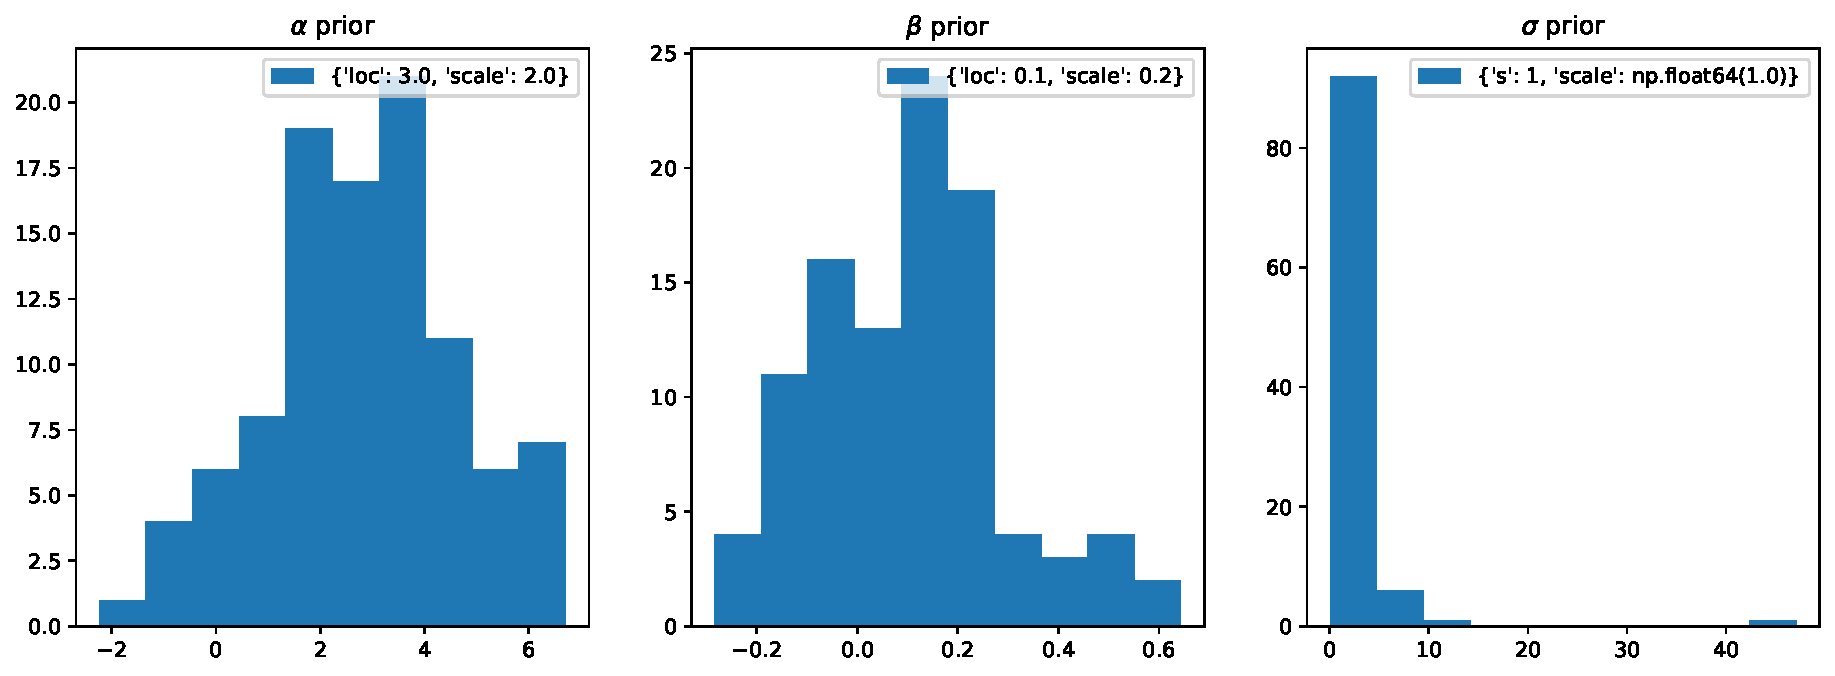
\includegraphics[width=\linewidth]{data/05_reporting/problem_set_2/prior_distributions.pdf}
    \caption{Prior distributions for the Linear Penguins model.}
    \label{fig:penguin-priors}
\end{figure}

\subsection{Prior-Predictive Verification}
\begin{figure}[H]
    \centering
    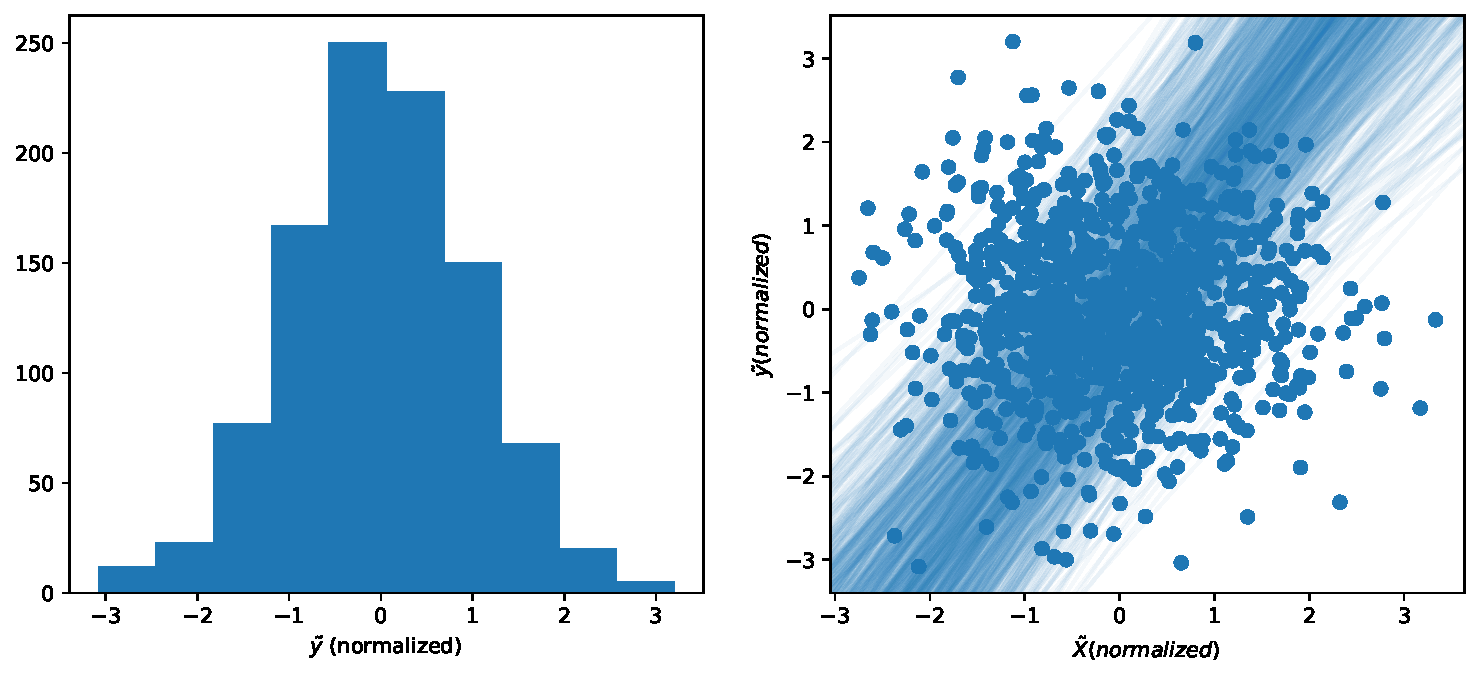
\includegraphics[width=0.8\linewidth]{data/05_reporting/problem_set_2/prior_predictive.pdf}
    \caption{Prior predictive distributions for $\tilde{y}$ and $\mu = \alpha + \beta X_i$ using bootstrapped $\tilde{X} \sim X_i$.}
    \label{fig:prior-predictive}
\end{figure}

Data are normalized before model fitting. Since this is linear regression, we would expect the largest mass of lines ($\mu = \alpha + \beta * X$) to have clear paths through the center of the data, as is seen in Figure \ref{fig:prior-predictive}.

\subsection{Posterior Distribution}

\subsection{Summarizing with Sample}

\subsection{Posterior Predictive}

\section{Building a MCMC Algorithm}

\subsection{Building Block: Proposal Distribution}

\subsection{Building Block: Acceptance}

\subsection{Putting it Together}

\subsection{Demonstration}

\subsection{Exploration (Optional)}

\end{document}
